\documentclass{article} % For LaTeX2e
\usepackage{nips13submit_e,times}
\usepackage{hyperref}
\usepackage{url}
\usepackage{amsmath}
\usepackage{graphicx,float,wrapfig}
\usepackage{caption}
\usepackage{subcaption}
%\documentstyle[nips13submit_09,times,art10]{article} % For LaTeX 2.09


\title{Probabilistic Matrix Factorization}


\author{ 
  Mert Terzihan \\
  Department of Computer Science\\
  Brown University\\
  Providence, RI 02912 \\
  \texttt{mert\_terzihan@brown.edu}
  \And
  Gabriel Barth-Maron \\
  Department of Computer Science \\
  Brown University \\
  Providence, RI 02912 \\
  \texttt{gabriel\_barth-maron@brown.edu}\\
}

% The \author macro works with any number of authors. There are two commands
% used to separate the names and addresses of multiple authors: \And and \AND.
%
% Using \And between authors leaves it to \LaTeX{} to determine where to break
% the lines. Using \AND forces a linebreak at that point. So, if \LaTeX{}
% puts 3 of 4 authors names on the first line, and the last on the second
% line, try using \AND instead of \And before the third author name.

\newcommand{\fix}{\marginpar{FIX}}
\newcommand{\new}{\marginpar{NEW}}

\nipsfinalcopy % Uncomment for camera-ready version

\begin{document}


\maketitle

\section{Description of the Problem}
\label{desc}
Matrix Factorization is a widely used method, especially in collaborative 
filtering and recommendation systems. With the rise of data available to 
researchers and the requirement to present personalized ads or recommendations 
to users led the researchers to further study of this field. As our final 
project, we will be dealing with Probabilistic Matrix Factorization on 
matrices with discrete values. 


\section{Discussion of Related Work}
\label{work}
As studied in [1] and [2], one can observe that LDA is equivalent to factorize a matrix 
probabistically using a graphical model representation. Instead of dealing with 
co-occurence matrix, we will try to propose a model and a learning algorithm to 
factorize a matrix where each cell is a rating of an item by a particular user. 
Therefore additional to LDA, we would also like to generate ratings that have been 
assigned by users to each item. 

[4] proposes a method based on LDA to produce personalized recommendations. 
However, fLDA takes into account many more information about the user, i.e. age, 
gender, zipcode, etc. We are going to use a simpler model, using only the rates 
that have been given by the users to specific items. 

[6] has proposed an LDA-based probabilistic matrix factorization model, however 
instead of using discrete distribution for generating ratings, it has placed a 
Gaussian distribution. 

\section{Graphical Model}
\label{graph}
Below is the graphical model and the details about it, where $j \in U$, $i \in M$ 
and $t \in T$, and $U$ is the total number of users, $M$ is the total number of items, 
and $T$ is the number of topics that we would like to extract. 
\begin{align*}
  &\theta_j \sim Dir(\alpha)\\
  &z_{ji} \sim Cat(\theta_j)\\
  &\phi_g \sim Dir(\beta)\\
  &x_{ji} \sim Cat(\phi_{z_{ji}}) \\
  &\kappa_{tj} \sim Dir(\gamma)\\
  &r_{ji} \sim Cat(\kappa_{z_{ji},j})
\end{align*}
\clearpage
\begin{figure}[h]
    \begin{center}
      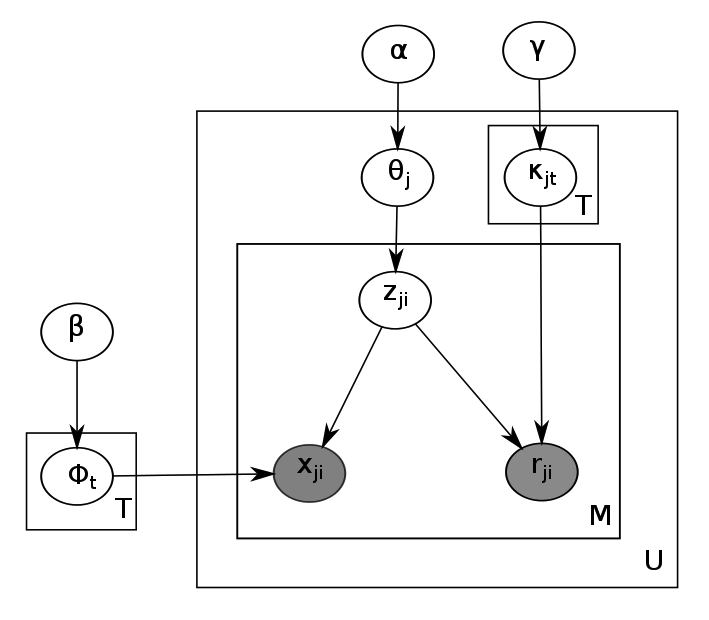
\includegraphics[width=.5\textwidth]{model.png}
      \caption{Representation of the Graphical Model}
      \label{fig:plot1}
    \end{center}
  \end{figure}

\section{Preliminary Experiment}
\label{exp}
[5]

\section{Learning Algorithm}
\label{alg}
MCMC and/or Variational Inference
Two ways to deal with incomplete data: 
\begin{itemize}
	\item 1) First complete the matrix and then factorize it
	\item 2) Operate on incomplete data likelihood as discussed in [3]
\end{itemize}

\section{Evaluation}
\label{eval}

\section{Timeline}
\label{time}

\subsubsection*{References}

\small{
[1] Blei, D.M., Ng, A.Y., and Jordan, M.I. Latent Dirichlet Allocation. In 
\textit{Journal of Machine Learning Research}, No. 2, pages 993-1022, March 2003. 

[2] Buntine, W., and Jakulin, A. Applying Discrete PCA in Data Analysis. In 
\textit{The Conference on Uncertainty in Artificial Intelligence}, 2004.

[3] Dempster, A.P., Laird, N.M., and Rubin, D.B. Maximum Likelihood from 
Incomplete Data via the EM Algorithm. In \textit{Journal of the Royal 
Statistical Society}, Series B, Vol. 39, No. 1, pages 1-38, 1977.

[4] Agarwal, D, and Chen, B. fLDA: Matrix Factorization through Latent Dirichlet 
Allocation. In \textit{The International Conference on Web Search and Data 
Mining}, 2010. 

[5] Kermarrec, A., and Moin, A. Data Visualization Via Collaborative Filtering. 
\textit{Research Report}, 2012, pp.23.

[6] Shan, H., and Banerjee, A. Generalized Probabilistic Matrix Factorizations for 
Collaborative Filtering. In \textit{IEEE International Conference on Data 
Mining}, 2010. 
}

\end{document}
